\documentclass[border=10pt]{standalone}

\usepackage{verbatim}

\usepackage{amsmath}
% my addons
\usepackage{graphicx}
%img path
\graphicspath{ {/home/propeller/Downloads/} }
%end of my addons


\usepackage[utf8]{inputenc}
\usepackage{tikz}
\usetikzlibrary{mindmap,shadows}
\usepackage[hidelinks,pdfencoding=auto]{hyperref}

% Information boxes
\newcommand*{\info}[4][16.3]{%
  \node [ annotation, #3, scale=0.65, text width = #1em,
          inner sep = 2mm ] at (#2) {%
  \list{$\bullet$}{\topsep=0pt\itemsep=0pt\parsep=0pt
    \parskip=0pt\labelwidth=8pt\leftmargin=8pt
    \itemindent=0pt\labelsep=2pt}%
    #4
  \endlist
  };
}


%Extra color defined 
\definecolor{tempGrn}{RGB}{0,153,153}
\definecolor{tempBlock}{RGB}{204,0,102}
\definecolor{tempSec}{RGB}{212,170,19}
%end of extra color

\begin{document}
\begin{tikzpicture}[ every annotation/.style = {draw,
                     fill = white, font = \Large}]
  \path[mindmap,concept color=black!40,text=white,
    every node/.style={concept,circular drop shadow},
    root/.style    = {concept color=black!70,
      font=\large\bfseries,text width=10em},
    level 1 concept/.append style={font=\Large\bfseries,
      sibling angle=45,text width=7.7em,
    level distance=25em,inner sep=0pt},
    level 2 concept/.append style={font=\bfseries,level distance=10em},
    level 3 concept/.append style={font=\bfseries,level distance=50em},
    level 4 concept/.append style={font=\bfseries, sibling angle=65,level distance=50em}
  ]
  node[root] {\huge Automatic Speech Rrecognition and TTS} [clockwise from=0]
    child[concept color=blue!60] {
      node (bitCore){{ASR}} [clockwise from=90]
    }
    child[concept color=blue, level distance=60em] {
      node[concept, text width = 10em] {{ \textbf{\textit{ASR} tasks}}(various dimensions)}
        [clockwise from=50]
      child[ level distance=20em] { node[concept, text width = 10em] (cc)
        {{Vocabulary Size}} }
      child [ level distance=15em]{ node[concept] (pk)
        {{Number of speaker}} }
      child [ level distance=15em]{ node[concept] (publicKeys)
        {{Channel and Noise} }
        % third child
        [clockwise from=340]
        child [level distance = 15em]{node[concept, text width = 10em](ellipticCurve) {{Accent}} }
        %end of third child
        }  
      child [ level distance=15em]{ node[concept, text width = 7em] (bitcoinAddress)
        {{ASR test, and training} }}    
    }
    child[concept color=green!40!black, level distance =55em] {
      node[concept](wallets) {{Waves to acoustics}}
        [clockwise from=260]
      child { node[concept, text width=9em] (nondet)
        {{Quantization}} }
      child { node[concept, text width=7em] (det)
        {{Sampling}}
       [clockwise from=210]
        child [level distance = 35em]{node[concept, text width = 10em]{{Feature extraction}} 
        [clockwise from=260]
        child [level distance = 20em]{node[concept, text width = 10em](hd) {{Windowing }}}
        child [level distance = 20em]{node[concept, text width = 10em](ms) {{DFT}}}
         child [level distance = 20em]{node[concept, text width = 10em](gm) {{MEL filter bank}}}
                }        
         }
    }
    child[concept color=tempGrn] {
      node[concept,text width =10em]  {{CTC}}
      [clockwise from=340]
      child { node[concept, text width=9em] (ds)
        {{Blank and allignment}} }
      child { node[concept, text width=7em](tFees) 
        {{CTC inference}}}
        child { node[concept, text width=7em](tIn)
        {{CTC Training}}}
        child { node[concept, text width=7em] (tOut)
        {{CTC and En-Dec}}}  
        child { node[concept, text width=7em] (utxo)
        {{Streaming models}}}     
    }   
    child[concept color=red!60!black, level distance= 60em] {
      node[concept] {{Other ASR Tasks}}
        [counterclockwise from=80]
      child { node[concept,text width = 9em] (pp)
        {{Wake word}}}
        child { node[concept,text width = 9em] (pp)
        {{Speaker diarization}}}    
      child { node[concept,text width = 7em] (nd)
        {{Spekar recognition}} }
        child { node[concept,text width = 7em] (nd)
        {{language identification}} }
    }
    child[concept color=tempBlock,level distance= 60em] {
      node[concept] (bc)
        {{ASR evaluation}}
        [clockwise from=200]
        child { node[concept](mt) {{Word error rate}}}
        child { node[concept,text width = 7em](gb) {{MAPSSWE}}}
        child { node[concept,text width = 7em] (bh){{MacNemar}}}
        }
    child[concept color=yellow!60!black, level distance=50em] {
      node[concept] (Blogs) {TTS} [clockwise from=120]
      child { node[concept, text width=8em](mining) {{Text normalizing}}}    
      child { node[concept,text width=8em] (dc){{Spectrogram prediction}} }  
    }
    child[concept color=tempSec, level distance = 50em] {
      node[concept,text width =10em] (Blogs) {Architecture} [clockwise from=50]
      child { node[concept, text width=8em](bprac) {{Encoder and decoder}} }
      child { node[concept, text width= 8em] (sp)
        {{Adding model}} }
    };
    %ASR 
    \info[30]{bitCore.north east}{above,anchor=west,xshift=1em}{%
      \item The general task of  \textbf{\textit{Automatic Speech Recognition (ASR)}} is to transform \textbf{\textit{wave form}} to appropriate \textbf{\textit{string of words}} .
      \vspace{1em}
      \item Where \textbf{\textit{keyboards}} are less convenient, \textbf{\textit{speech}} acts as main form of interface. i.e \textit{ smart home appliances, personal assistants, or cellphones}.
      \vspace{1em}
      \item \textbf{\textit{ASR}} is integral part of \textbf{\textit{augmentative communication}}.
    }
    %End of ASR
    
    % bitcoin network
    \info[20]{pp.north west}{above,anchor=south, xshift=3em, yshift= 3em}{%
      \item The detection of \textbf{\textit{short word or phrase}}.
      \vspace{1em}
      \item \textbf{\textit{Wake word}} detection needs to be \textbf{\textit{fast, small}} which can be stored in a embeded systems.
    }
     \info[25]{nd.south west}{below,anchor=north}{%
      \item \textbf{\textit{Speaker verification, speaker identification}} are closely related to \textbf{\textit{language identification}}.
      \vspace{1em}
      \item A speaker language must be autometically identified to chosse appropriate operations.
    }
    %end of bitcoin network
    \info[20]{nondet.south}{below,anchor=north,xshift=5em}{%
      \item The size of \textbf{\textit{quant}} is either \textbf{\textit{8 bits}} or \textbf{\textit{16 bits}}.
      \vspace{1em}
      \item All vaules that are closer together than the \textbf{\textit{minimum granularity}} are represented identically.
      \vspace{1em}
      \item The norm is to denote each sample as \textbf{\textit{n}}, where as it \textit{quantized} waveform as \textbf{\textit{x[n]}}
    }
    
    \info[23]{wallets.south}{above, anchor=west, yshift=5em,xshift=4em}{%
      \item The first task in  \textbf{\textit{ASR}} is to convert input waveform to bunch of \textbf{\textit{feature vectors.}} 
      \vspace{1em}
      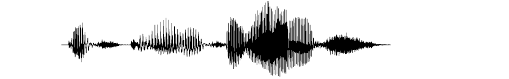
\includegraphics[scale=.6]{images/wave}      
      \item We normally get \textbf{\textit{analog}} representation of voices.
      \vspace{1em}
      \item From that \textbf{\textit{analog}} represantation, we separate \textbf{\textit{analong input from microphone}} and \textbf{\textit{air pressure}}.
      \vspace{1em}
      \item Finally, we convert this two to \textbf{\textit{digital signal.}}
    }
    \info[20]{det.west}{anchor=east, yshift=-15em}{%
      \item  A \textbf{\textit{ signal}} is sampled by measuring its \textbf{\textit{amplitude}} at a \textbf{\textit{particular time}}.
      \vspace{1em}
      \item The \textbf{\textit{sampling rate}} is samples taken \textbf{\textit{per second.}}
      \vspace{1em}
      \item We must need \textbf{\textit{two samples}} in each cycle to measure wave accurately. One is \textbf{\textit{positive part}} of the wave, and the other one is \textbf{\textit{negative part}} of the wave.
      \vspace{1em}
      \[ \begin{cases} 
      rate > 2  & higher~accuracy \\
	 rate < 2  & completly~missed \\
   \end{cases}
	\]
       \vspace{1em}
       \item The maximum frequency for a given \textbf{\textit{sampling rate}} is called \textbf{\textit{Nyquist frequency}}.
       \vspace{1em}
       \begin{itemize}
       	\item \textbf{\textit{10,000 Hz}} to \textbf{\textit{20,000 Hz}} for human speech.
       	\item \textbf{\textit{8,000 Hz}} for telephone-bandwith speech.
       	\item \textbf{\textit{16,000 Hz}} for Microphone speech.
       \end{itemize}
       \item One important note is that we need to \textbf{\textit{downsmaple}} while \textbf{\textit{normalizing}} when we work with multiple corpora from different dimensons.
    }
    \info[30]{pk.south east}{above,anchor=north west}{%
      \item \textbf{\textit{Read Speech}} is relatively easier to recognize. For example when human speaking to a machine, or reading out loud etc.
      \vspace{1em}
      \item \textbf{\textit{Conversational Speech}}, in which two people talks with each other is very hard to recognize.
    }
    
    
    \info[22]{bitcoinAddress.south}{below,anchor=north,xshift=-3em}{%
\item[]A few human-created transcripts that are used to create \textbf{\textit{ASR test and training}}.
\vspace{1 em}
     \item \textbf{\textit{LibriSpeech}} is an \textit{open-source} \textit{read-speech} \textbf{\textit{16 kHz}} datatset with the length of \textbf{1000 hours} audio.
     \vspace{1em}
     \item The \textbf{\textit{Switchboard}} corpus is collection of \textbf{\textit{telephone}} coversations, collected in early 1990s, each one averaging 6 minutres; totaling 240 hours of \textbf{\textit{8 kz}}. They did hand-done linguistic labeling. 
     \vspace{1em}
     \item The \textbf{\textit{CALLHOME}} corpus was collected in  the early 1990, has coversation of native speakers with their friends, each one is roughly 30-minutes.
     \item \textbf{\textit{CORAAL}} is a collection of over  150 \textbf{\textit{sociolinguistic}} interviews with African American speakers. Transcripts are aligned at utterance level. 
     \item\textbf{\textit{CHiME}} has been designed to test \textbf{\textit{robustness}} in ASR. This libraray has collection of speech in real home evironment \textit{kitchen, dining area, living room} with \textit{four} participants of \textit{twenty} different dinner parties.
     \item \textbf{\textit{HKUST}} is collection of 1206 \textit{ten-minutes} telephone speech in \textit{mandarian}.
     \item \textbf{\textit{AISHELL-1}} contains dialects from northern China, taken from various domains, nearly 170 hours worth of content.
    }
    
    
    \info[20]{publicKeys.south west}{below,anchor=north,yshift=-1em}{%      
 \item This one is trivial, it is always harder to read from a speaker who is talking from far, or in a crowded street, on the other hand it is easier to read when we record something in a quite room, with proper recording setups.
    }
    
    
 
    
    \info[30]{cc.east}{anchor=west,xshift = 0.5em}{%
      \item  \textbf{\textit{Two words}} vocabulary \textit{(i.e yes, no)}, and \textbf{\textit{ eleven words}} vocabulary \textit{(i.e: numbers)} are solved with extreamly high accuracy.
      \vspace{1em}
      \item Human speech or conversation transscribtion which has \textbf{\textit{60,000}} words are much harder harder task.
    }
    \info[20]{ellipticCurve.south}{anchor=west, xshift=5em}{%
    \item If we train our model in standard dialect systems, it will be trivially harder to recognize regional dialect. Form that we can also conclude, if we train an model using only adult speaker it will be difficult to read from children voice.                     
          }
          
          
          %hd wallet info......................
           \info[30]{gm.south}{anchor=east, xshift=-5em,yshift=10em}{%
      \item Humen are biased to \textbf{\textit{low frequencies}}, it helps us extract crucial \textbf{\textit{values or nasals}}.
      \vspace{1em}
       \item To implement this intution we collect \textbf{\textit{enegies}} of waves, not in each \textbf{\textit{band}}, rather according to \textbf{\textit{mel}} scale.
       \vspace{1em}
       \item A \textbf{\textit{mel}} is a \textbf{\textit{unit}} of \textbf{\textit{pitch}}. Each sounds that are \textbf{\textit{perceptually equidistant}} are separated by an equal \textbf{\textit{number of mels}}.
       \item[] \begin{equation*}
       	mel(f) = 1127 \ln (1+\frac{f}{700})
       \end{equation*}
       \vspace{1em}
       \item We spread everything \textbf{\textit{logarithmically}} so that we have accurate resolution at \textbf{\textit{low frequency}} and less at \textbf{\textit{high frequecny}}. It discards \textbf{\textit{noises}}, \textbf{\textit{power variations}}.                
          }
      \info[30]{ms.south}{anchor=east, xshift=-5em}{%
      \item \textbf{\textit{Windowing}} is kind of discretization of a continous signal. To extract \textbf{\textit{spectral}} infromation from a \textbf{\textit{discrete frquency}} bands for a \textbf{\textit{discrete-time}} signal is the \textbf{\textit{discrete Forurier transform}}.
      \vspace{1em}
      \item So the \textbf{\textit{input}} to the DFT is a windowed signal $x[n] \cdots x[m]$.
      \vspace{1em}
      \item The \textbf{\textit{output}} is a \textbf{\textit{complex}} number $X[k]$ reperesenting \textbf{\textit{magnitude}} and \textbf{\textit{phase}}.    
}
\info[45]{hd.south}{anchor=north, xshift=-5em}{%
\item At this stage we have \textbf{\textit{digitized}}, and \textbf{\textit{quantized}} representation of \textbf{\textit{analog}} wave form. Now we need to extract \textbf{\textit{spectral}} features from a small \textbf{\textit{window}} which corresponds to a singale \textbf{\textit{phoneme}}.
\vspace{1em}
\item Inside this small window we consider signal as \textbf{\textit{stationary}} signal, although our speech is by nature \textbf{\textit{non-stationary}}. Speech extracted from this window is called a \textbf{\textit{frame}}.
\vspace{1em}
\item The windowing is characterized by \textbf{\textit{three}}
parameters.
\begin{itemize}
\item The \textbf{\textit{window size}} or\textbf{\textit{frame size}}. 
\item The \textbf{\textit{frame stride}}.
\item The \textbf{\textit{shape}} of the window.
\end{itemize}
\item[] To extract the signal we multiply the value of the signal at time \textbf{\textit{n}}, \textbf{\textit{s[n]}} by the value of the window at time \textbf{\textit{n}},\textbf{\textit{w[n]}}.
\item[] \begin{equation*}
 y[n] = w[n]s[n]
 \end{equation*}
\vspace{1em}
\item In \textbf{\textit{winowing}} technique we abruptly cutt-off signal from adjacent region, which creates malfunction during \textbf{\textit{Fourier}} analysis. For this reason \textbf{\textit{Hamming}} window comes to play, it \textbf{\textit{shrinks}} value around the region instead of total cut-off.
\vspace{1em} 
 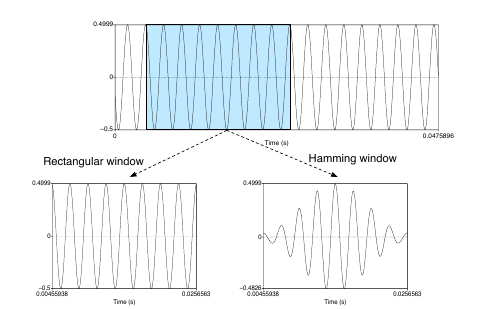
\includegraphics[scale=.9]{images/hamming}
 \vspace{1em}
 \item The equations that governed \textbf{\textit{rectangular}} window, and \textbf{\textit{hamming}} window are as follows
 \begin{itemize}
 \item rectangular window
  \[ \begin{cases} 
      1  & 0\leq n \leq L-1 \\
	 0  & otherwise \\
   \end{cases}
	\]	
	\item Hamming window
	  \[ \begin{cases} 
      0.54-0.46cos(\frac{2\pi n}{L})  & 0\leq n \leq L-1 \\
	 0  & otherwise \\
   \end{cases}
	\]
 \end{itemize}
\vspace{1em}
}


%end of hd wallet info.............................

% transaction info
\info[25]{utxo.north west}{above,anchor=south,xshift=2em}{%
     \item Since \textbf{\textit{CTC}} does not wait for sentence to be finished like \textbf{\textit{Endcoder-decoder architechture}}, we can use it for \textbf{\textit{streaming}}.
     \vspace{1em}
     \item To serve \textbf{\textit{stremaing}} we need to use \textbf{\textit{RNN-T}} with \textbf{\textit{CTC}}.
    }
    
    
    \info[20]{tOut.north west}{above,anchor=south,xshift = -6em}{%
      \item We can combine both \textbf{\textit{CTC architectures}} and \textbf{\textit{Encoder-decoder}}.
      \vspace{1em}
    \item For training, we will add \textbf{\textit{two losses}} with weighted $\lambda$ on a \textbf{\textit{dev set}}.
    }
    
    \info[30]{tIn.west}{anchor=east, yshift=-5em}{%
      \item To train a \textbf{\textit{ASR}} using \textbf{\textit{CTC}} we use \textbf{\textit{negative log-likelihood}} loss function with a special \textbf{\textit{CTC loss function}}.
      \vspace{1em}
      \item We use \textbf{\textit{forward-backward algorithm}} to merge allignments dynamically as well as increase the efficiancy of \textbf{\textit{sum over all probabilities}}.
    }
    
 \info[30]{tFees.south}{anchor=north, xshift=3em}{%
\item \textbf{\textit{CTC}} is special algorithimic technique to compensate our naive approach by introducing \textbf{\textit{blanks and allignment}}.
\vspace{1em}
\item We \textbf{\textit{allign}} each input $x_{i}$ at time $t$ with each output $\hat{y_{i}}$, thus we get rid off \textbf{\textit{decoder}}.
\vspace{1em}
\item We consider \textbf{\textit{all the allingments}} for probabable output, but it can give us errornous result, so we use \textbf{\textit{sum over all}}, but this \textbf{\textit{sum over all}} is costly, so we use \textbf{\textit{special beam search}}.
}
%end transaction info

% blockchain info
\info[25]{bh.north east}{above,anchor=west,xshift=1em}{%
      \item This one is also like \textbf{\textit{MAPSSWE}}, but it compares errors when two systems are \textbf{\textit{independent}} of eacth other.
    }
 \info[30]{mt.south}{anchor=east, xshift=-2em,yshift=5em}{%
     \item \textbf{\textit{Word error rate}} is the standard metric for evaluating \textbf{\textit{ASR}}. To do this we compare \textbf{\textit{hypothesized}} word string with \textbf{\textit{reference}} word string.
      \vspace{1em}
      \item We use \textbf{\textit{minimum distance algorithm}} to build the metric, mainly to find word \textbf{\textit{substitutions}}, word \textbf{\textit{insertions}}, word \textbf{\textit{deletions}} in order to map between \textbf{\textit{hypothesized}} words, and \textbf{\textit{correct word}}.
      \vspace{1em}
      \item []\begin{equation*}
      	WER = 100 \times \frac{Insertion+del + subs}{Total~ correct ~words}.
      \end{equation*}
      \vspace{1em}                        
          }
          
\info[30]{gb.south}{anchor=east, xshift=2em,yshift=10em}{%
      \item  \textbf{\textit{MAPSSWE}} is a \textbf{\textit{parametric test}} that compares between two different \textbf{\textit{systems}}.              
          }
          
 
 % end of blockchain info
 %mining info
  \info[30]{mining.south}{anchor=east, xshift=-2em,yshift=15em}{%
      \item \textbf{\textit{Text normalization}} is needed for handling \textbf{\textit{non-standard}} words, non-standard words are defined as  \textbf{\textit{numbers, monetary amounts, dates etc. }}
      \vspace{1em}
      \item  \textbf{\textit{Seniotic class}} is the criteria that helps us to find meaning of non-standard words in a sysmatic way.
      \vspace{1em}
      \item  \textbf{\textit{Text- noramlization}} can be done in two ways.
      \begin{itemize}
      \item Rule-based normalization
      \item Endcoder-decoder based normalization.
      \end{itemize}
      \item To address more complex systems we use lightweight  \textbf{\textit{covering grammers}}.
          }
          \info[30]{dc.north east}{above,anchor=west,xshift=1em}{%
      \item \textbf{\textit{Spectrogram prediction}} is the attention based encode-decoder architecture for TTS.
      \vspace{1em}
      \item The whole processes are as follows:
      \begin{itemize}
      \item The \textbf{\textit{encoder}} takes sequence of letters as input, and produces hidden representation which later used by \textbf{\textit{decoder}}. These whole thing then passed through \textbf{\textit{3 convolutional}} layers, each conataing \textbf{\textit{512 filters}}.
      \vspace{1em}
      \item In \textbf{\textit{Decoder}}, the prior trained \textbf{\textit{mel}} spectrum has passed as a \textbf{\textit{bottleneck}}. The system is trained on \textbf{\textit{gold log-mel}} filterbank features.
\end{itemize}       
    }
 % end of mining info
 % security info
 \info[30]{sp.east}{anchor=south west, yshift=-20em}{%
      \item The \textbf{\textit{scoring}} is in each language model is done with weight $\lambda$ tuned on held out set, and \textbf{\textit{normalizing}} the probability by \textbf{\textit{number of characters}} in the hypothesis $|Y|_{c}$.
      \vspace{1em}
      \item[]\begin{equation*}
       score(Y|C) = \frac{1}{|Y|_{c}} \ln P(Y|X) + \lambda log P_{LM}(Y)
      \end{equation*}
      \item The loss is probality of \textbf{\textit{correct token}}.
      \vspace{1em}
      \item The loss of \textbf{\textit{entire stentence}} then beomes \textbf{\textit{sum of each token losses}}.
      \vspace{1em}
      \item In these model, we use \textbf{\textit{teacher}} forcing to correct \textbf{\textit{gold}} $y_{i}$ rather than predicted $\hat{y_{i}}$.
    }
     \info[40]{bprac.north west}{above,anchor=south, xshift=5em}{%
      \item \textbf{\textit{Implemented with RNN or Transformer}}
      \vspace{1em}
      \item \textbf{\textit{Attention- based encoder decoder or AED }}
      \vspace{1em}
      \item \textbf{\textit{One vector per 10 ms frame}}
      \vspace{1em}
      \item \textbf{\textit{$y\in \lbrace a, b, c, \cdots, 0,9, \langle space \rangle, \langle comma \rangle,\langle period \rangle, \langle apostrophe \rangle, \langle unk \rangle$}}
      \vspace{1em}
      \item \textbf{\textit{Subsampling}}
      \vspace{1em}
      \item \textbf{\textit{Output via greedy decoding}}
       \vspace{1em}
      \item[] $\hat{y} = argmax_{char \in Alphabet}P(char|y_{1}\cdots y_{i-1},X)$         
      \vspace{1em} 
    }
    %end security info
    
    %extra info
    \info[85]{det.west}{anchor=east, xshift=45em, yshift=-68em}{%
      \item \textbf{{\huge Semiotic Class For Detecting Non-Standard Words}}
      \vspace{2em}
      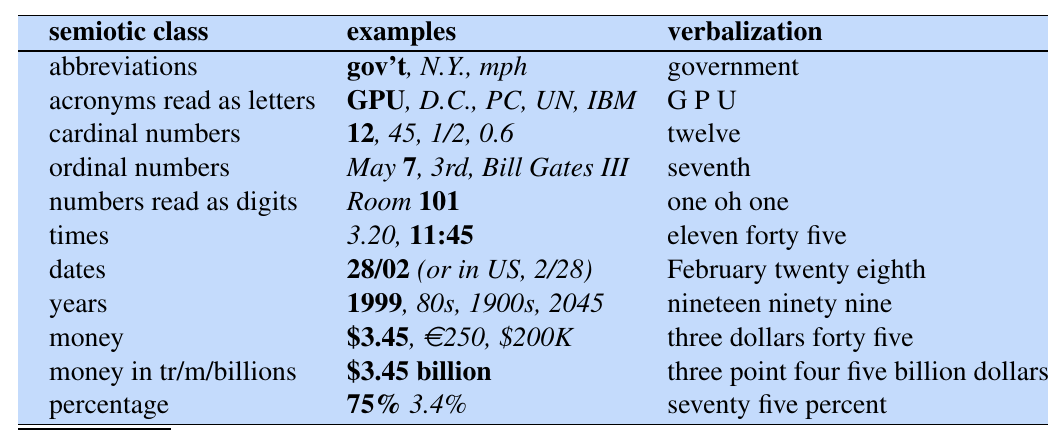
\includegraphics[scale=1]{images/semiotic}
    }
    \info[85]{ellipticCurve.south}{anchor=west, yshift=-60em, xshift=-5em}{%
    \item \textbf{\huge Encoder-Decoder Architecture}\\
    \vspace{1em}
       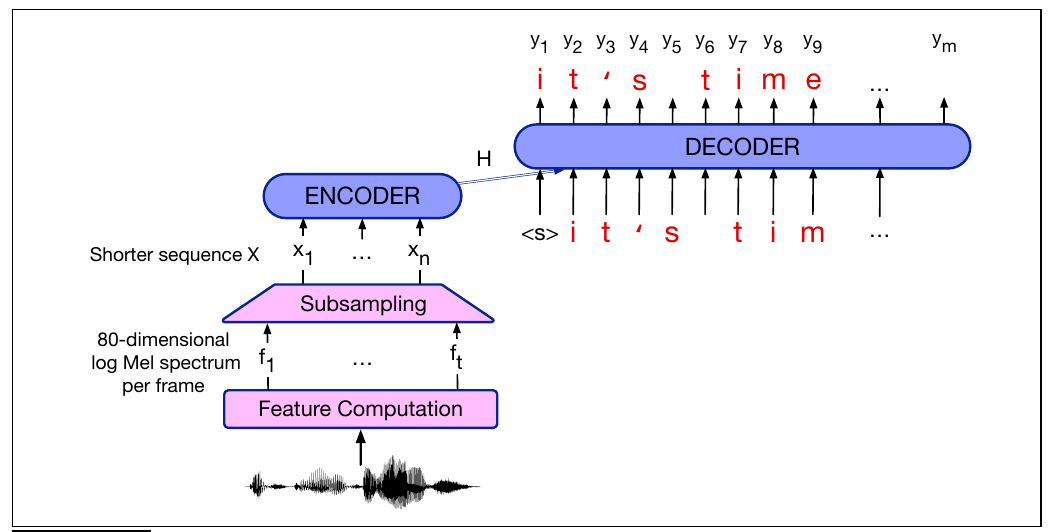
\includegraphics[scale=1]{images/endcoder}                      
     \item \textbf{\huge Inference with CTC}
     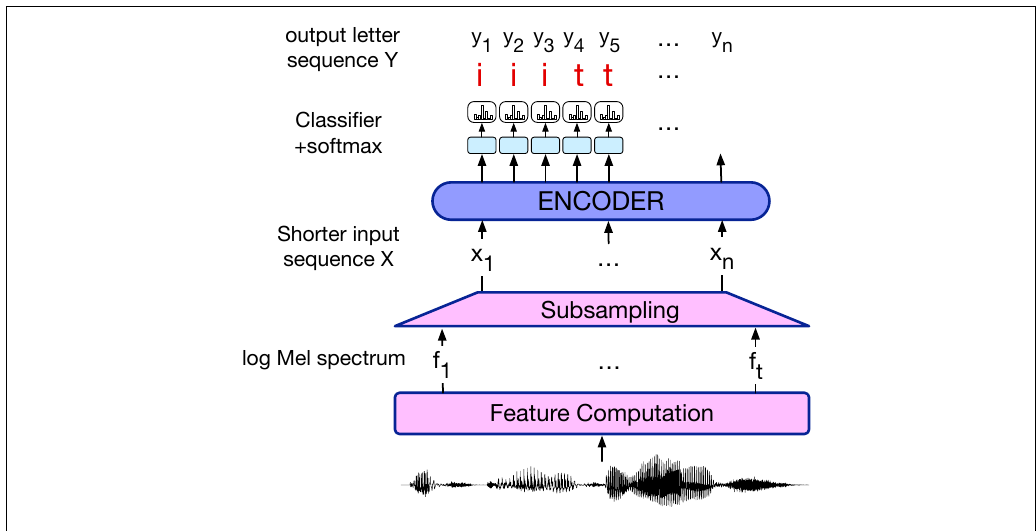
\includegraphics[scale=1]{images/ctc}                      
          }
          \info[50]{dc.north east}{above,anchor=west,xshift=70em, yshift= 10em}{%
      \item \Huge MD. Galib Ahsan
      \vspace{1em}
      \item \Huge ID: 20166062
    }
\end{tikzpicture}
\end{document}

